\documentclass[11pt]{amsart}
%\geometry{landscape}                % Activate for for rotated page geometry
\usepackage[parfill]{parskip}    % Activate to begin paragraphs with an empty line rather than an indent
\usepackage{graphicx, txfonts} %txfonts makes the letters sharp
\DeclareGraphicsRule{.tif}{png}{.png}{`convert #1 `dirname #1`/`basename #1 .tif`.png}
\usepackage{epstopdf}
\usepackage{mathtools}
\usepackage{hyperref}
\usepackage{amsthm, amssymb, amsfonts, amsmath, enumerate}
\usepackage{mathrsfs} %Needed for \mathscr
\usepackage{relsize}%, xfrac} % for resizing in math mode




\graphicspath{ {/home/TaylorHeilman/Desktop/CS335/hw7} }\begin{document}

\title[CS/MATH 335 HW 7]{CS/MATH 335: Probability, Computing, and Graph Theory \\ Homework 7\\ Due in class Tuesday, November 8, 2016}
\maketitle

{Taylor Heilman and Matt Iammarino}

\textbf{Partner Problems}

Roughly in order of difficulty

\begin{enumerate}

\item \fbox{\parbox{\textwidth}{
Mitzenmacher 5.18}} 
{



}

\item \fbox{\parbox{\textwidth}{
Mitzenmacher 5.17
}}

{


 
}

\item \fbox{\parbox{\textwidth}{
Mitzenmacher 5.19 
}}

{


 }
\item \fbox{\parbox{\textwidth}{
Bollobas
}}

{



}










\item[(5)] \fbox{\parbox{\textwidth}{
Individual
}} 
{
a.) This problem consists of two parts. First you must create an arrangement of edges in-between the two sets (no two vertices in a set are adjacent) of $n=2k$ vertices  which makes a $k$ coloring possible. Second, you must create an ordering of the vertices which creates a $k$ coloring of the graph. This can be done by placing $k$ vertices in each set. Number each vertex in set 1 and 2 with the labels $1,2,3,...,k-1,k$. Create an edge between all vertices which are not labeled the same number. The ordering of the vertices to obtain a $k$ coloring is as following: Start with any vertex from set 1 and color it, then color the vertex from set 2 that it is not adjacent to.  Pick another vertex from set 1 that is not already colored and color it and then color the non adjacent vertex from set 2. Repeat these steps until all vertices are colored.  The resulting coloring of the graph will be $k$ colored. See the pictures below for a visual of the graphs and their ordering for the greedy algorithm. 
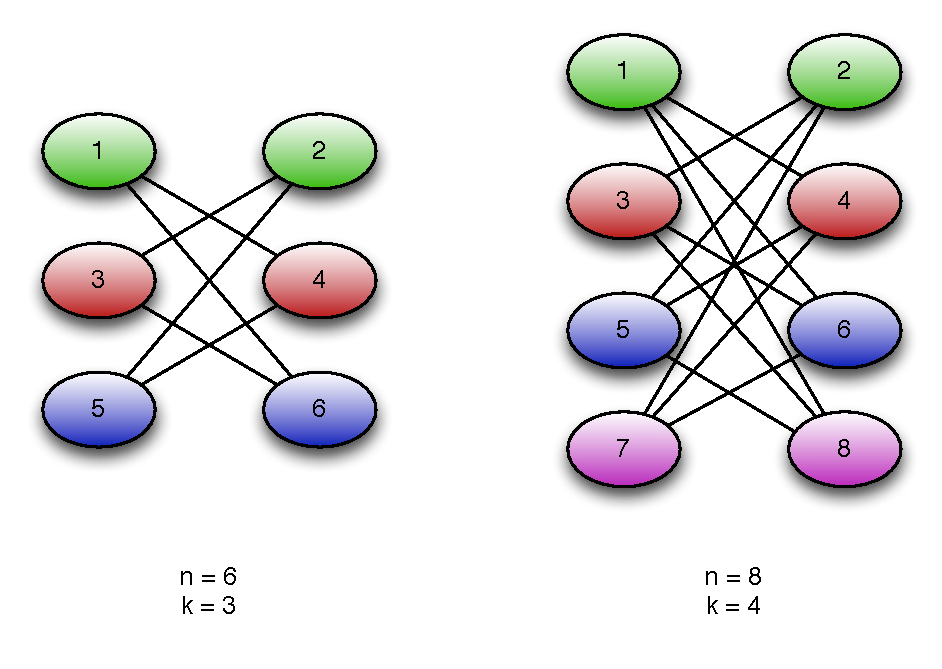
\includegraphics[scale=.5]{colorings}



b.) This can be done with $n=2k-2$ vertices.  First put $\frac{n}{2}$ vertices in each set. Follow the same algorithm as above except the final 2 vertices of either set are now adjacent to all $\frac{n}{2}$ vertices of the opposite set. Following the same order as above will result in a $k$ coloring when $n=2k-2$.  See the pictures below.

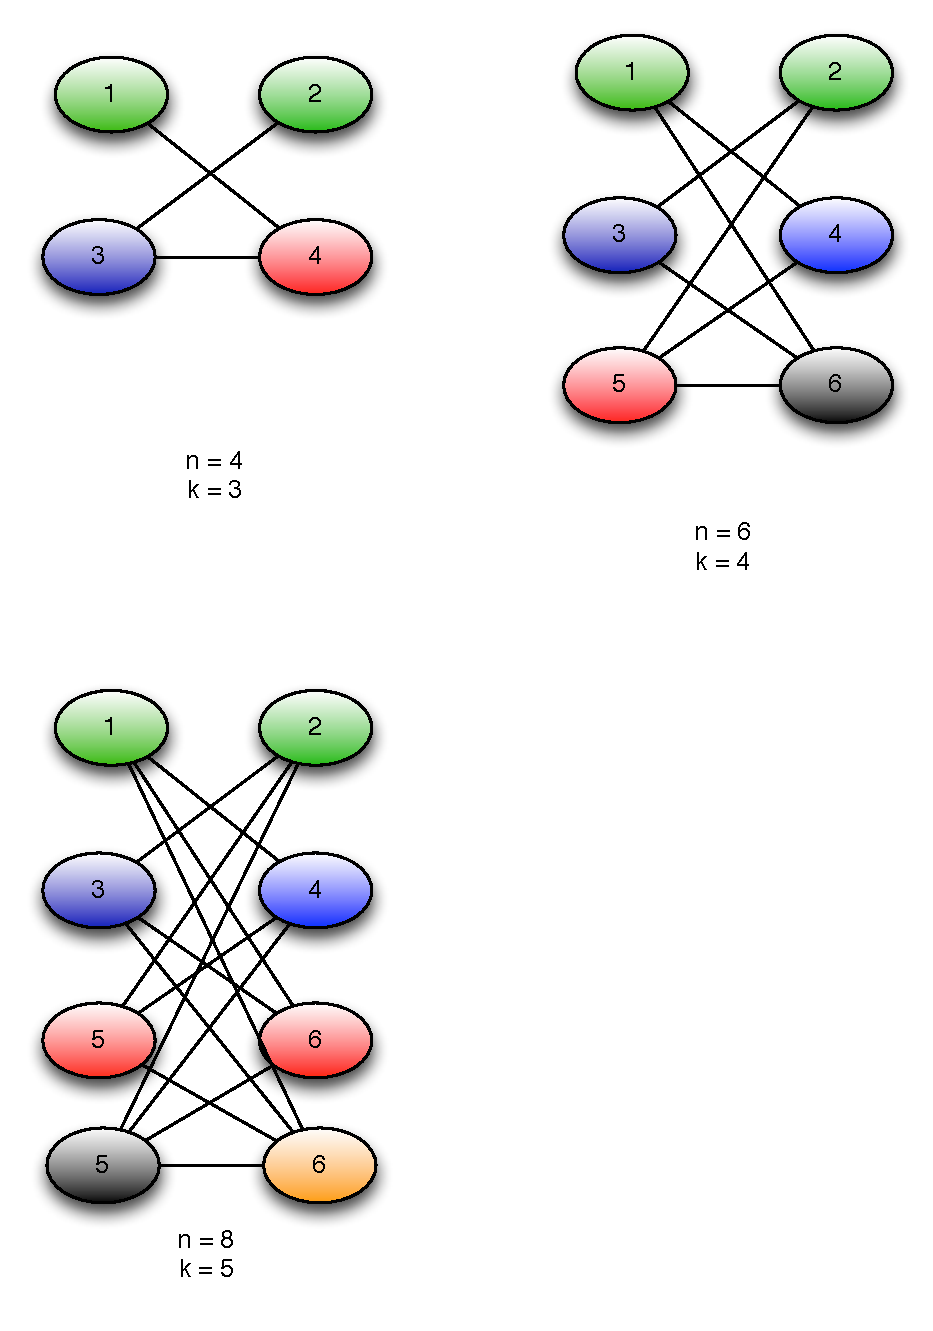
\includegraphics[scale=.5]{colorings2}


c.) We can prove that a $k $ coloring does not exist for $n=2k-3$ vertices by looking at the case where $k = 3$, which gives us $n = 3$.  By the pigeon hole principle one set will have 1 vertex, WLOG assume the first set has 1 vertex.  We have $3!$ possible orderings on the graph.  All 6 possible orderings are shown below and all result in a 2 coloring.  This result occurs because whenever a bipartite graph has only one vertex in a set the maximal coloring of the graph is 2.

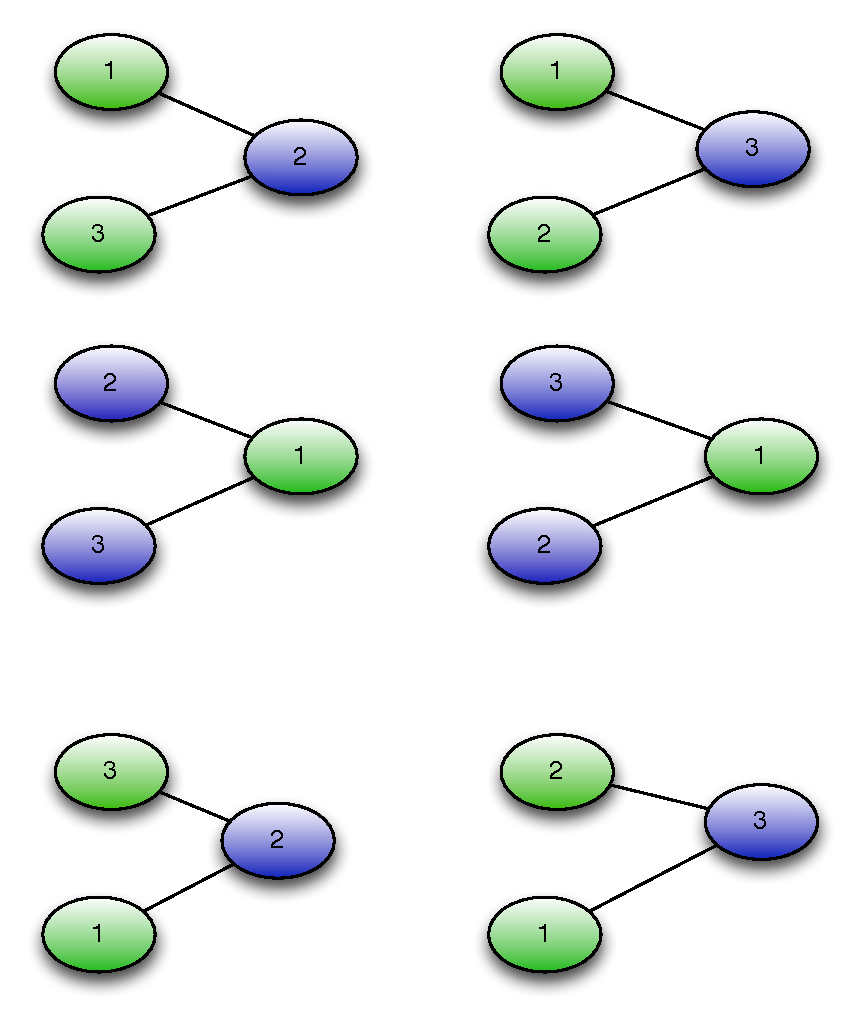
\includegraphics[scale=.5]{colorings3}




}



\item[(6)] \fbox{\parbox{\textwidth}{
Individual Bonus problem

}} 

{



}


\end{enumerate}

\end{document}